\section{System}\label{sec:system}

\subsection{Overview}
Figure~\ref{fig:architecture} shows the components. A \emph{gateway} sits between the agents and the shared artifacts and tools; it stamps every served copy and keeps a registry. The edit log (and, when available, the read log and the registry) feed an \emph{audit} that calls copies, links reads to uses, and produces a \emph{trace graph} with an evidence tier on every edge. The graph yields an attribution for each output and a re-check list. A \emph{benchmark harness} runs swarms in a sandbox, keeps the hidden read log as the answer key, and scores any tracer that sees only what a real investigator would. A local \emph{viewer} draws the trace graph as an ant colony for human inspection. Every component except the gateway works on logs that already exist.

\begin{figure}[t]
\centering
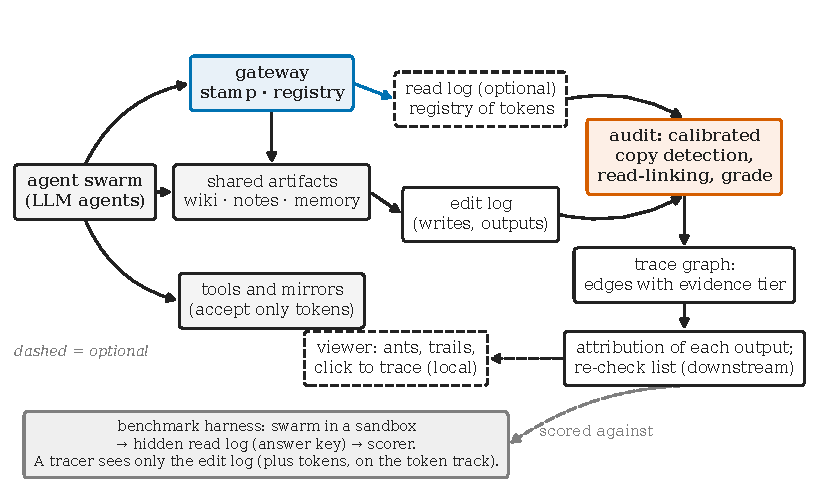
\includegraphics[width=\linewidth]{figures/fig_architecture.pdf}
\caption{Components and data flow. Dashed boxes are optional: the audit works on the edit log alone, and uses the read log and the registry when they exist. The benchmark harness scores a tracer against the hidden read log.}
\label{fig:architecture}
\end{figure}

\subsection{The audit: calibrated copy detection}\label{sec:audit}
The audit takes a log with fields agent, time, channel and content (other shapes are mapped to these) and answers: if something bad spread through this swarm, could it be traced? Algorithm~\ref{alg:audit} extracts distinctive strings, calls copies only where a string is strong evidence, and reports carrier coverage (Definition~\ref{def:coverage}).

\begin{algorithm}[t]
\caption{Calibrated copy detection}\label{alg:audit}
\begin{algorithmic}[1]
\Require events $E$ sorted by time, each $(a,t,c,x)$ = (agent, time, channel, content); $N_{\max}=\maxAgents{}$
\State $\mathrm{first}\gets$ empty map: token $\mapsto$ agent $\mapsto (t,c)$
\For{each event $(a,t,c,x)$ in $E$}
  \For{each $w\in\textsc{Tokens}(x)$}
    \State \textbf{if} $a\notin\mathrm{first}[w]$ \textbf{then} $\mathrm{first}[w][a]\gets(t,c)$
  \EndFor
\EndFor
\For{each token $w$ with $|\mathrm{first}[w]|\ge2$}
  \State $(\kappa,\sigma)\gets\textsc{Classify}(w)$;\quad order its users by first-use time as $u_1,u_2,\dots,u_n$
  \State $\mathrm{trusted}\gets n\le N_{\max}\ \wedge\ \kappa\notin V\ \wedge\ (\sigma=\text{high}\ \vee\ n\le3)$
  \For{$k=2,\dots,n$}
    \State $\mathrm{carriers}\gets\{u_j:\ j<k,\ \mathrm{channel}(u_j)=\mathrm{channel}(u_k)\}$
    \State emit $(w,u_k,\mathrm{carriers},\mathrm{trusted})$
  \EndFor
\EndFor
\State $\mathrm{coverage}\gets\big|\{\text{trusted rows with carriers}\}\big|\,/\,\big|\{\text{trusted rows}\}\big|$; grade by Table~\ref{tab:grade}
\end{algorithmic}
\end{algorithm}

\textsc{Tokens} are runs of at least 12 characters from $[\mathrm{A\text{-}Za\text{-}z0\text{-}9\_\text{-}}]$ after URL-decoding up to three times and removing redaction markers, kept only if they are not common words or headers, not long hex or digit runs, have at least seven distinct characters, and contain a digit, mixed case or an underscore. \textsc{Classify} labels a token as a UUID, a high-entropy identifier (Shannon entropy at least $3.3$ bits per character), a timestamp, a snake\_case or camelCase identifier, or other; $V$ is the set of vocabulary classes (snake\_case and camelCase identifiers and round, constructed timestamps), which agents type independently and which are never trusted. A string is \emph{trusted} when it is used by at most $N_{\max}=\maxAgents{}$ agents, is not vocabulary, and is either strong evidence (a UUID or minted identifier) or used by at most three agents. This is the practical counterpart of the base-rate test of Proposition~\ref{prop:calib}; Section~\ref{sec:res-real} uses the explicit likelihood-ratio test on the real incident. The audit also reports the \emph{best possible top-1} (Corollary~\ref{cor:uniform}), the strings that many agents type (``everyone types this''), naive against calibrated counts, and what to log next. When no trusted copy exists it reports N/A rather than a grade: a log in which agents share nothing distinctive proves nothing about traceability.

\begin{table}[t]
\centering\small
\caption{Grade thresholds on carrier coverage (Definition~\ref{def:coverage}).}\label{tab:grade}
\begin{tabular}{@{}lccccc@{}}
\toprule Grade & A & B & C & D & F \\ \midrule coverage $\ge$ & \gradeA\% & \gradeB\% & \gradeC\% & \gradeD\% & below \\ \bottomrule
\end{tabular}
\end{table}

The audit runs as a command-line tool and as a browser page that reads the file locally and sends nothing anywhere; a parity test requires the two to agree on counts, grade and shared-string tables on all test files, including samples of real logs.

\subsection{Linking reads to uses}\label{sec:links}
If the log has read events, Algorithm~\ref{alg:links} links an agent's first later event that contains something it read to the author of what it read. The most specific matching read wins, so a short tagless link inside a longer tagged one is not a second candidate. If no exact copy matches, the \emph{weak} tier matches the same link with its tag, token or query stripped: the agent used what it read, but not the copy it was served, so which copy is unknown. The tiers are reported separately because they carry different evidence.

\begin{algorithm}[t]
\caption{Read-linking}\label{alg:links}
\begin{algorithmic}[1]
\Require sorted events; read events carry (reader, time, served content, source author)
\For{each agent $a$ and its first non-read event $e$ that contains something $a$ read earlier}
  \State $H\gets\{r\in\mathrm{reads}_a\text{ before }e:\ |r.\mathrm{content}|\ge12,\ r.\mathrm{source}\ne a,\ r.\mathrm{content}\subseteq e.\mathrm{content}\}$
  \If{$H\ne\emptyset$} \State remove from $H$ every $r$ whose content is a proper substring of another member's content;\ $\mathrm{weak}\gets\textbf{false}$
  \Else \State $H\gets\{r:\ \textsc{Strip}(r.\mathrm{content})\subseteq\textsc{Strip}(e.\mathrm{content})\}$;\ $\mathrm{weak}\gets\textbf{true}$
  \EndIf
  \If{$H\ne\emptyset$} \State $\mathrm{sources}\gets$ distinct authors in $H$;\ emit $(a,\mathrm{sources},\ \mathrm{exact}=(|\mathrm{sources}|=1\wedge\neg\mathrm{weak}),\ \mathrm{weak})$
  \EndIf
\EndFor
\end{algorithmic}
\end{algorithm}

\subsection{The canary gateway}\label{sec:gateway}
Algorithm~\ref{alg:gate} is the gateway of Proposition~\ref{prop:gate}. The design space has two axes. \emph{Granularity}: a token per served copy (version-unique), per origin, or per page; Proposition~\ref{prop:tags} says only the first identifies the immediate source. \emph{Necessity}: an \emph{inert} tag is decoration (a query parameter the mirror ignores) that a copier can drop without penalty; a \emph{load-bearing} token is part of what the link needs to work (a session segment the mirror requires). Section~\ref{sec:res-survival} shows that necessity matters and that it matters differently for different models. In the lab, the inert condition appends a random-looking query value to every served link, and the load-bearing condition re-mints a fresh valid session token in every served link. A gateway also needs \emph{closure}: if the resource server hands a session to anyone who asks, an agent can bypass the token; the gated condition removes that route (Section~\ref{sec:res-gate}).

\begin{algorithm}[t]
\caption{Canary gateway}\label{alg:gate}
\begin{algorithmic}[1]
\Procedure{Serve}{reader $r$, version $v$, time $t$}
  \For{each chunk $i$ of $v$ and each link $\ell$ in chunk $i$}
    \State $\tau\gets$ fresh random token;\quad $R[\tau]\gets(r,v,i,\mathrm{author}_i,t)$
    \State replace any token already in $\ell$ by $\tau$ \Comment{a copied token is never reused}
  \EndFor
  \State \Return the stamped text
\EndProcedure
\Procedure{Accept}{request $q$}
  \State $\tau\gets\textsc{TokenIn}(q)$;\quad \textbf{if} $\tau\in\mathrm{dom}(R)$ \textbf{then forward} $q$ \textbf{else refuse}
\EndProcedure
\Procedure{Resolve}{$\tau$} \State \Return $R[\tau]$ \EndProcedure
\end{algorithmic}
\end{algorithm}

\subsection{Re-check sets}\label{sec:recheck}
Given an origin $o$, Algorithm~\ref{alg:recheck} follows trace edges forward and returns the downstream set. Edges from hidden sources and from coincidences are not followed, so the list never relies on a guess; this is conservative where the log is silent. The comparison lists in Section~\ref{sec:res-tip} are: everything after the item appeared, the earliest-writer rule, tokens alone, and tokens with the earliest-writer rule as the fallback where a token was lost.

\begin{algorithm}[t]
\caption{Re-check set (downstream)}\label{alg:recheck}
\begin{algorithmic}[1]
\Require trace edges $(u\to v,\ \mathrm{kind})$ with $\mathrm{kind}\in\{$exact, one-of-several, weak, string-in-room, hidden, coincidence$\}$; origin $o$
\State $\mathrm{out}\gets\emptyset$;\quad queue $\gets[o]$
\While{queue not empty}
  \State pop $u$;\ \textbf{for} each edge $(u\to v,\mathrm{kind})$ with $\mathrm{kind}\notin\{\text{hidden},\text{coincidence}\}$ and $v\notin\mathrm{out}\cup\{o\}$: add $v$ to $\mathrm{out}$ and to the queue
\EndWhile
\State \Return $\mathrm{out}$
\end{algorithmic}
\end{algorithm}

\subsection{Benchmark and viewer}\label{sec:benchsys}
The benchmark exports each lab run in three parts: the \emph{edit-log view} that a real investigator would have, the \emph{hidden truth} (which copy each agent was served), and, for the token track, the \emph{registry}. A standard-library scorer reports the metrics of Definition~\ref{def:tracer} with run-level bootstrap intervals and ships five baselines (Appendix~\ref{app:bench}). The viewer is a local page that runs the same tracing core as the audit and draws each agent as an ant in a chamber for its room, with trails for trace edges; clicking an ant shows its trace back and its downstream set. It makes no network request and masks strings from the log by default.

\paragraph{Cost.} The audit is linear in the number of tokens in the log; read-linking is linear in events times reads per agent; the downstream search is linear in the trace graph. The gateway adds a random token and a registry write per served link.
